% !TEX root = ../../main.tex

\chapter{Mean-Field and Dynamic Mean-Field Theory}
\label{ch:mean-field-dynamic-mean-field-theory}

\section*{What This Chapter Adds}

Chapter~\ref{ch:random-rate-networks-scs-chaos} showed the core SCS move: a
large random recurrent network can be replaced by a representative stochastic
unit, but only if the statistics of that unit reproduce the statistics assumed
for its input. This chapter develops that idea systematically. Static mean-field
theory describes stationary firing rates and stationary mean input. Dynamic
mean-field theory (DMFT) describes autocorrelations, effective noise processes,
and the distinction between finite-size fluctuations and quenched disorder.

The goal is to make the clustered spiking roadmap mathematically legible. We
want to understand when a \(Q\)-cluster excitatory/inhibitory network reduces
to equations for representative cluster activities, why stationary balance is
not enough to decide whether the state is multistable or chaotic, and how the
autocorrelation \(C(\tau)\) becomes a self-consistency object.

\section{Static Mean Field: Matching Mean Inputs}
\label{sec:ch07-static-mean-field}

Mean-field theory begins with a deliberate loss of detail. Instead of tracking
all neuron-to-neuron inputs, we replace many microscopic variables by their
population averages. For a population \(\alpha\in\{E,I\}\), let
\[
        r_\alpha = \left\langle A_\alpha(t)\right\rangle
\]
be its stationary mean firing rate. A static transfer function gives
\[
        r_\alpha = \Phi_\alpha(\mu_\alpha),
        \label{eq:ch07-static-transfer}
\]
where \(\mu_\alpha\) is the stationary mean input to population \(\alpha\).
This is a self-consistency equation: \(\mu_\alpha\) is computed from the rates,
and the rates are computed from \(\mu_\alpha\).

For a clustered E/I network with cluster index \(a\), a schematic mean input is
\[
        \mu_a^\alpha
        =
        I_\alpha^{\mathrm{ext}}
        +
        \sum_{\beta\in\{E,I\}}
        \widehat J^{\alpha\beta}n_\beta r_a^\beta
        +
        \sum_{b\ne a}
        \sum_{\beta\in\{E,I\}}
        \check J_{ab}^{\alpha\beta}n_\beta r_b^\beta .
        \label{eq:ch07-cluster-mean-input}
\]
The first term is external drive. The second term is input from the same
cluster, with intra-cluster weights \(\widehat J^{\alpha\beta}\). The third term is
input from other clusters, with inter-cluster weights
\(\check J_{ab}^{\alpha\beta}\). The factors \(n_\beta\) appear because
population activity is an average, while synaptic input sums over presynaptic
neurons.

In the sparse subpopulation setup from the roadmap, every population receives a
fixed in-degree \(K\) of external cluster inputs, with \(K\ll Q\) in the sparse
large-network regime. Of these inputs, \(K_E=fK\) are excitatory and
\(K_I=(1-f)K\) are inhibitory. The external excitatory weight scale is
\(\check J\), while the external inhibitory weight scale is
\(-\check g\check J\), with
\[
        \check g=\frac{fg}{1-f}.
        \label{eq:ch07-check-g-definition}
\]
This choice keeps the external E/I cancellation in the same \(n_E-g n_I\) form
after the unequal numbers of external E and I inputs are counted:
\[
        fK\,n_E r-\check g(1-f)K\,n_I r
        =
        fK\left(n_E-g n_I\right)r .
\]
Under the additional stationary assumptions used in the roadmap calculation,
excitatory and inhibitory cluster activities have the same mean rate \(r\), and
the scalar covariance formulas below use a symmetric activity-covariance
simplification: the connected E and I activity autocovariances are represented
by one \(C_A(\tau)\), while E/I cross-covariances are not kept at this scalar
level. With these assumptions, the stationary mean synaptic input takes the form
\[
        \bar{y}
        =
        \left(\widehat J+\check J fK\right)
        \left(n_E-g n_I\right)r .
        \label{eq:ch07-roadmap-stationary-input}
\]
Here \(g\) is the inhibitory strength relative to excitation after this
\(\check g\) rescaling. The expression displays the balanced-network idea in
compressed form: excitation and inhibition are both large, and the net mean
input depends on their cancellation.

Static mean field answers the necessary compatibility question of whether the
proposed stationary rates match the recurrent input they generate. It does not
answer the dynamic question of whether rate fluctuations decay, switch between
attractors, or become chaotic. DMFT is the dynamic extension.

\section{Why Self-Consistency Is More Than Averaging}
\label{sec:ch07-self-consistency}

A mean-field equation is self-consistent when the object assumed on the input
side equals the object produced on the output side. Static mean field enforces
this equality for means:
\[
        r_\alpha
        =
        \Phi_\alpha\!\left(
        I_\alpha^{\mathrm{ext}}+
        \sum_\beta W_{\alpha\beta}r_\beta
        \right).
        \label{eq:ch07-static-self-consistency}
\]
DMFT enforces the analogous equality for time-dependent second-order
statistics. If \(C_\alpha(\tau)\) is the autocovariance of population or cluster
activity,
\[
        C_\alpha(\tau)
        =
        \left\langle
        A_\alpha(t)A_\alpha(t+\tau)
        \right\rangle
        -
        r_\alpha^2,
        \label{eq:ch07-activity-autocovariance}
\]
then the theory must compute the input covariance from the activity covariance
and then require the representative population to reproduce that same
\(C_\alpha(\tau)\).

This is why the SCS equation
\[
        \left\langle \eta(t)\eta(t+\tau)\right\rangle
        =
        g^2 C_r(\tau)
\]
is not merely a definition of noise. It is a closure condition. The network is
allowed to generate irregular input only if a unit driven by that input returns
the activity statistics used to generate it.

\section{Quenched and Annealed Disorder}
\label{sec:ch07-quenched-annealed}

The roadmap separates two sources of variability that can look similar in a
single trace but scale differently.

\begin{description}
    \item[Finite-size variability.]
    A cluster rate averages over finitely many spike trains. Its amplitude
    scales as
    \[
        \xi = \frac{1}{\sqrt{n_E}} .
        \]
    Increasing the number of excitatory neurons per cluster reduces this source
    of fluctuations.

    \item[Quenched variability.]
    Inter-cluster couplings are drawn once and then held fixed. The parameter
    \(\kappa\) denotes the strength of this frozen variability, for example
    heterogeneity in \(\check J_{ab}^{\alpha\beta}\) or random cluster-level
    connectivity. Increasing \(n_E\) does not average it away if the same
    cluster-to-cluster disorder remains.
\end{description}

The word \emph{quenched} means frozen in time. A quenched matrix is sampled at
network construction and then kept fixed while the dynamics runs. The word
\emph{annealed} means redrawn in time, across trials, or across an averaging
procedure. Annealed noise may be useful as an approximation to some statistics,
but it removes the fixed recurrent structure that gives deterministic chaos its
sensitivity to initial conditions.

\begin{figure}[htbp]
    \centering
    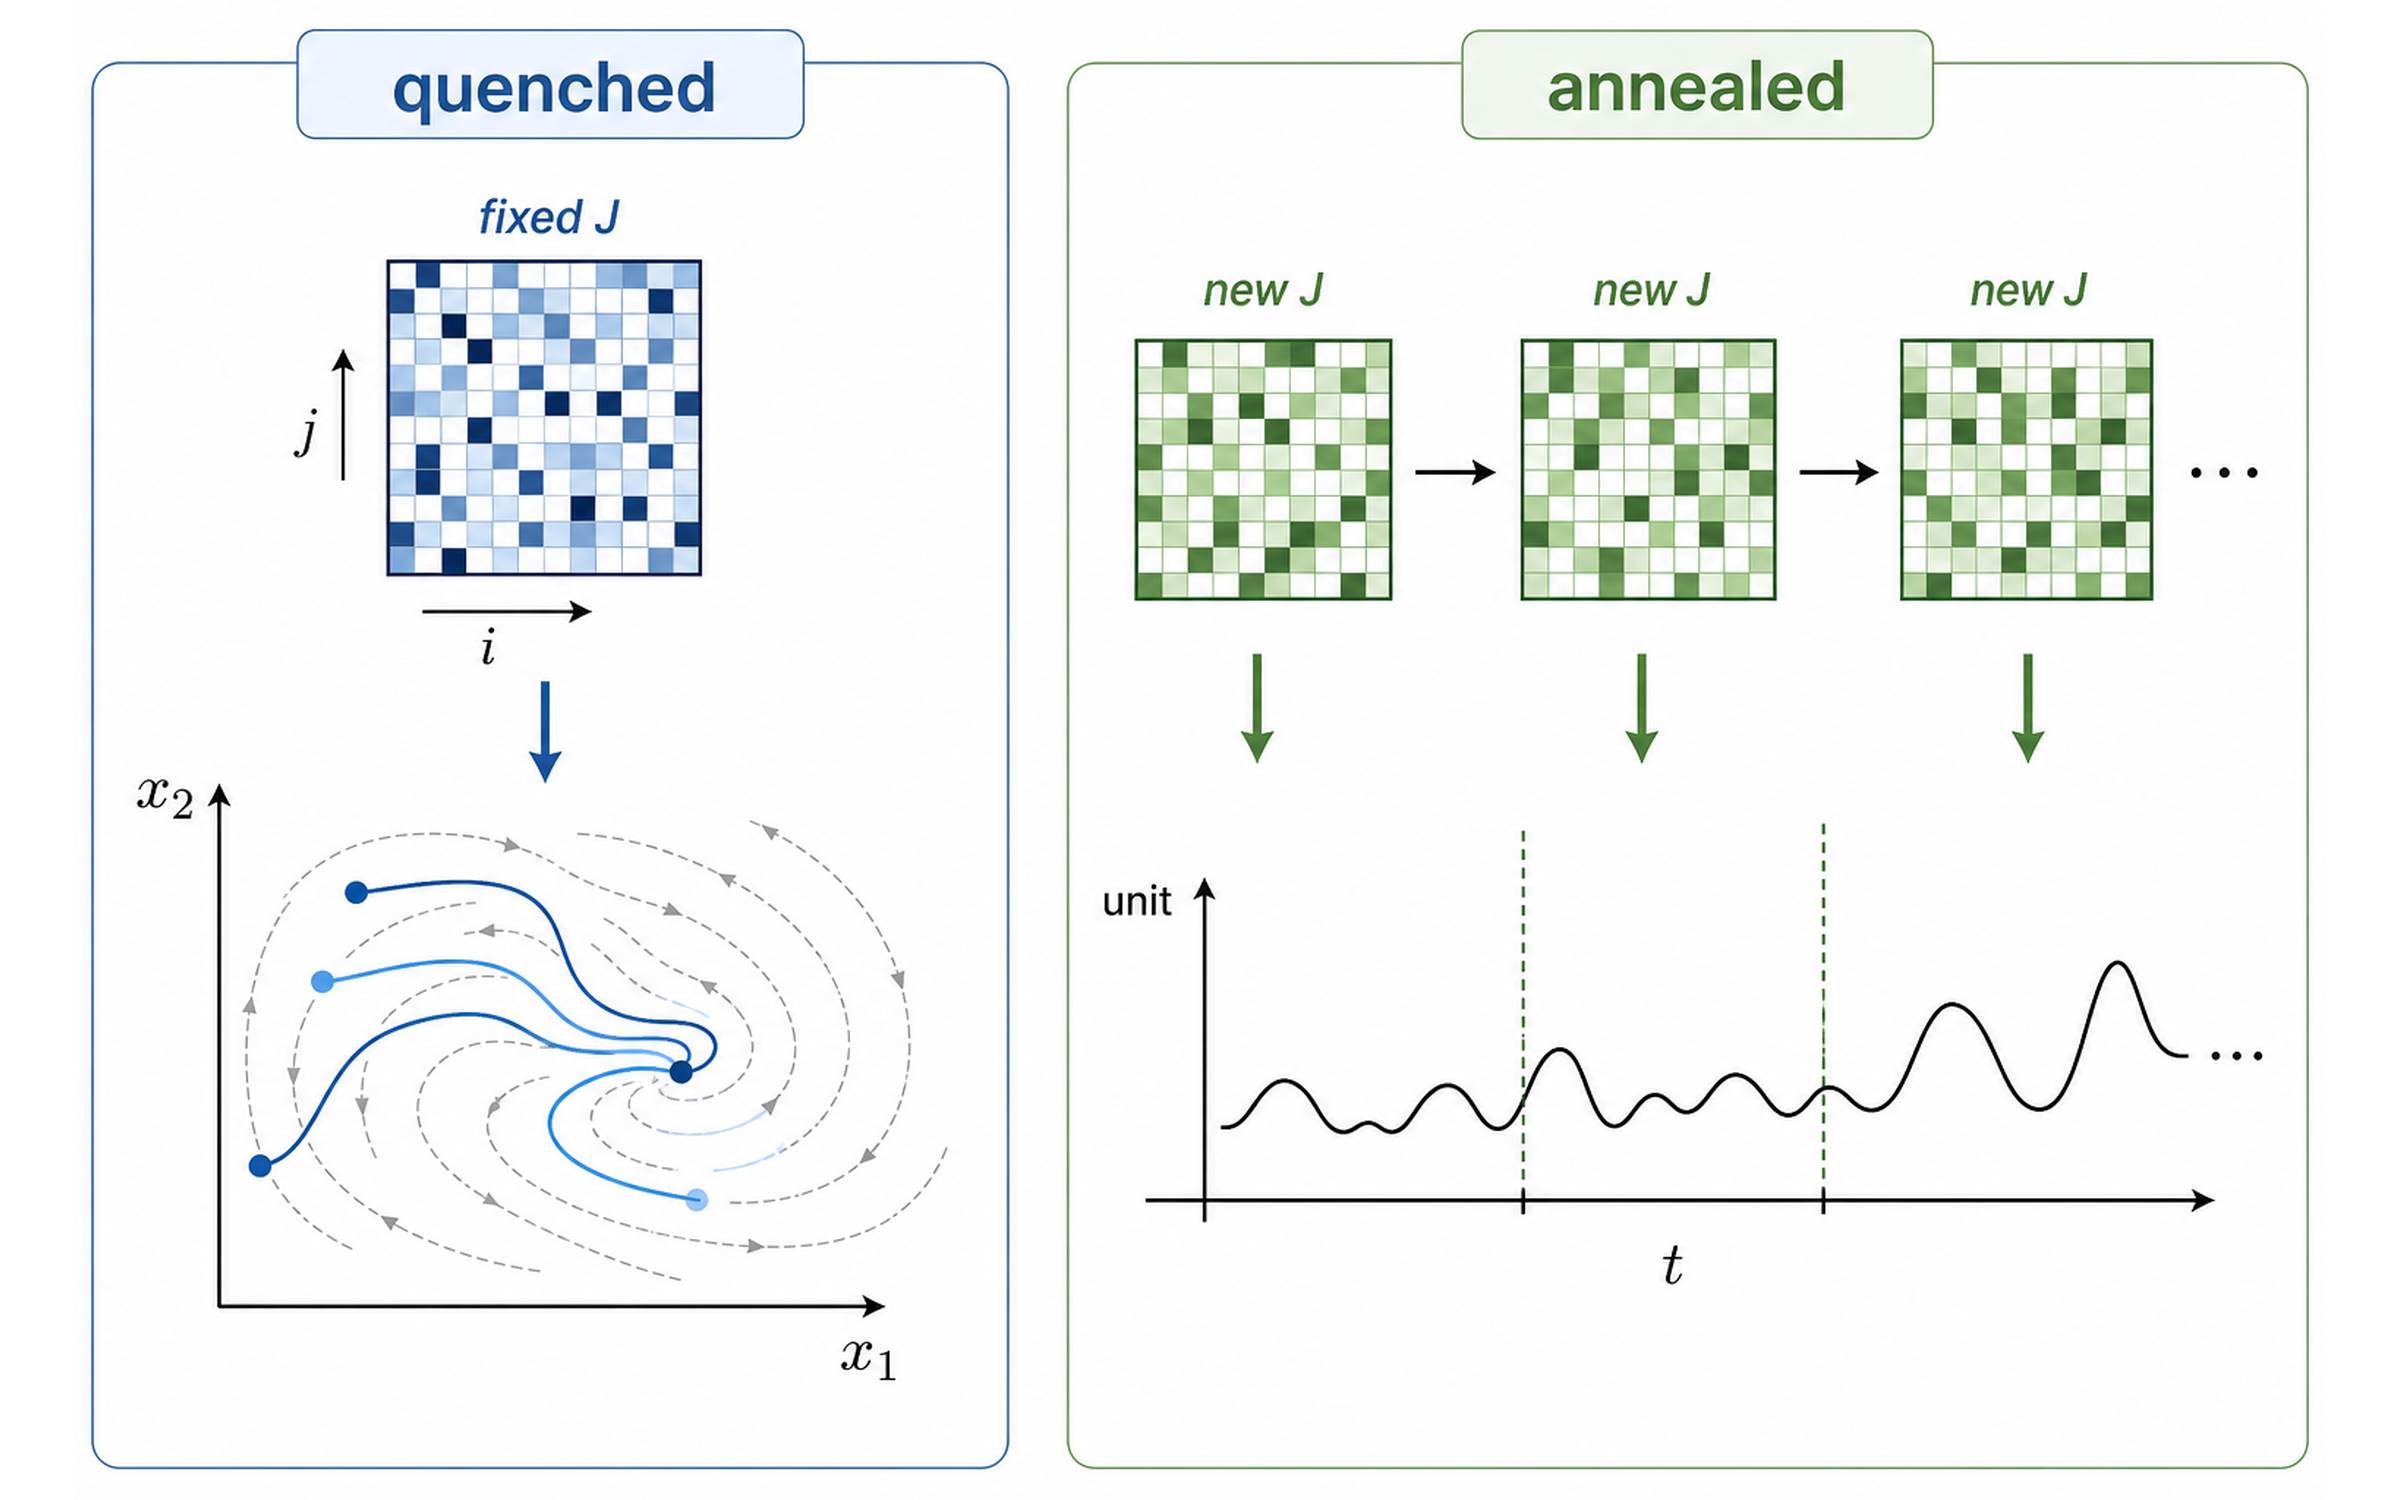
\includegraphics[width=0.88\textwidth]{figures/imagegen/ch07-quenched-vs-annealed-disorder-img.png}
    \caption{Quenched versus annealed disorder. Quenched inter-cluster weights
    are sampled once and remain part of the deterministic vector field, so the
    same frozen matrix shapes every trajectory. Annealed disorder is redrawn
    over time or trials; it can mimic an input variance but not the fixed
    recurrent geometry responsible for deterministic sensitivity and Lyapunov
    growth.}
    \label{fig:ch07-quenched-vs-annealed-disorder}
\end{figure}

\begin{keyequation}[Quenched Structure Versus Annealed Finite-Size Forcing]
\begin{equation}
        \frac{d\mathbf u}{dt}
        =
        F(\mathbf u;\Delta_{\mathrm{q}})
        +
        \xi\,B(\mathbf u)\boldsymbol\eta(t),
        \qquad
        \Delta_{\mathrm{q}}\hbox{ fixed during a run.}
        \label{eq:ch07-quench-anneal-state-equation}
\end{equation}
\tcblower%
\(\Delta_{\mathrm{q}}\) denotes frozen inter-cluster weights, sparse adjacency,
or heterogeneous depression factors. It changes the deterministic vector field
and is controlled by \(\kappa\). The process \(\boldsymbol\eta(t)\) represents
finite population sampling fluctuations; its amplitude is controlled by
\(\xi\). Perturbation tests for chaos must keep \(\Delta_{\mathrm{q}}\) fixed
and, when possible, use common finite-size noise.
\end{keyequation}

Equation~\eqref{eq:ch07-quench-anneal-state-equation} is the operational
distinction behind the later diagnostics. If a simulation redraws the quenched
matrix between two nearby trajectories, it is no longer measuring sensitivity
to initial conditions in one dynamical system. If it redraws finite-size noise
independently, it measures stochastic divergence rather than deterministic
Lyapunov growth. Conversely, if \(\Delta_{\mathrm{q}}\) is held fixed and
\(\xi\) is reduced by increasing cluster size, any persistent irregularity must
come from the deterministic or quenched mesoscopic part of the model.

\section{The DMFT Effective Process}
\label{sec:ch07-effective-process}

Consider again a random rate network, now allowing a nonzero mean output. A
representative unit can be written as
\[
        \tau_r \frac{d x}{dt}
        =
        -x(t) + \mu + \eta_0 + \zeta(t),
        \qquad
        r(t)=\phi(x(t)).
        \label{eq:ch07-dmft-effective-rate}
\]
The deterministic mean input is
\[
        \mu = J_0 m + I,
        \qquad
        m = \left\langle \phi(x(t))\right\rangle .
        \label{eq:ch07-dmft-mean}
\]
The random recurrent part must now be split into two pieces. The static
quenched bias \(\eta_0\) is constant in time for a given representative unit,
but varies across units or disorder realizations:
\[
        \left\langle \eta_0 \right\rangle = 0,
        \qquad
        \left\langle \eta_0^2 \right\rangle = g^2m^2,
        \qquad
        \left\langle \eta_0\zeta(t) \right\rangle=0 .
        \label{eq:ch07-dmft-static-quenched-bias}
\]
The dynamic fluctuation \(\zeta(t)\) has zero mean and connected covariance
\[
        \left\langle \zeta(t)\zeta(t+\tau)\right\rangle
        =
        g^2 C_r(\tau),
        \label{eq:ch07-dmft-noise-covariance}
\]
where
\[
        C_r(\tau)
        =
        \left\langle
        \phi(x(t))\phi(x(t+\tau))
        \right\rangle
        -
        m^2 .
        \label{eq:ch07-dmft-output-covariance}
\]
is the connected output autocovariance. Equivalently, the total random recurrent
input \(\eta_0+\zeta(t)\) has covariance based on the raw second moment
\[
        Q_r(\tau)
        =
        \left\langle
        \phi(x(t))\phi(x(t+\tau))
        \right\rangle
        =
        m^2+C_r(\tau),
        \qquad
        \left\langle
        \bigl(\eta_0+\zeta(t)\bigr)
        \bigl(\eta_0+\zeta(t+\tau)\bigr)
        \right\rangle
        =
        g^2Q_r(\tau).
        \label{eq:ch07-dmft-raw-moment}
\]
The terms have distinct jobs. The time constant \(\tau_r\) sets the filtering
time of the representative rate variable. The mean \(\mu\) is the static
mean-field input. The static random variable \(\eta_0\) records the frozen
projection of the nonzero mean activity through random weights. The process
\(\zeta(t)\) records dynamic recurrent fluctuations around that bias. If
\(m=0\), the static component vanishes and the compact SCS covariance
\(\langle \eta(t)\eta(t+\tau)\rangle=g^2C_r(\tau)\) is recovered.

Equations~\eqref{eq:ch07-dmft-effective-rate}--\eqref{eq:ch07-dmft-raw-moment}
are DMFT in its compact rate-network form. They contain three matching
requirements: the mean input must match the mean output, the connected dynamic
input covariance must match the connected output autocovariance multiplied by
the coupling variance, and the raw recurrent input covariance must include the
static quenched contribution \(g^2m^2\) when \(m\ne0\). The representative unit
must be driven by the same process it helps create.

\begin{figure}[htbp]
    \centering
    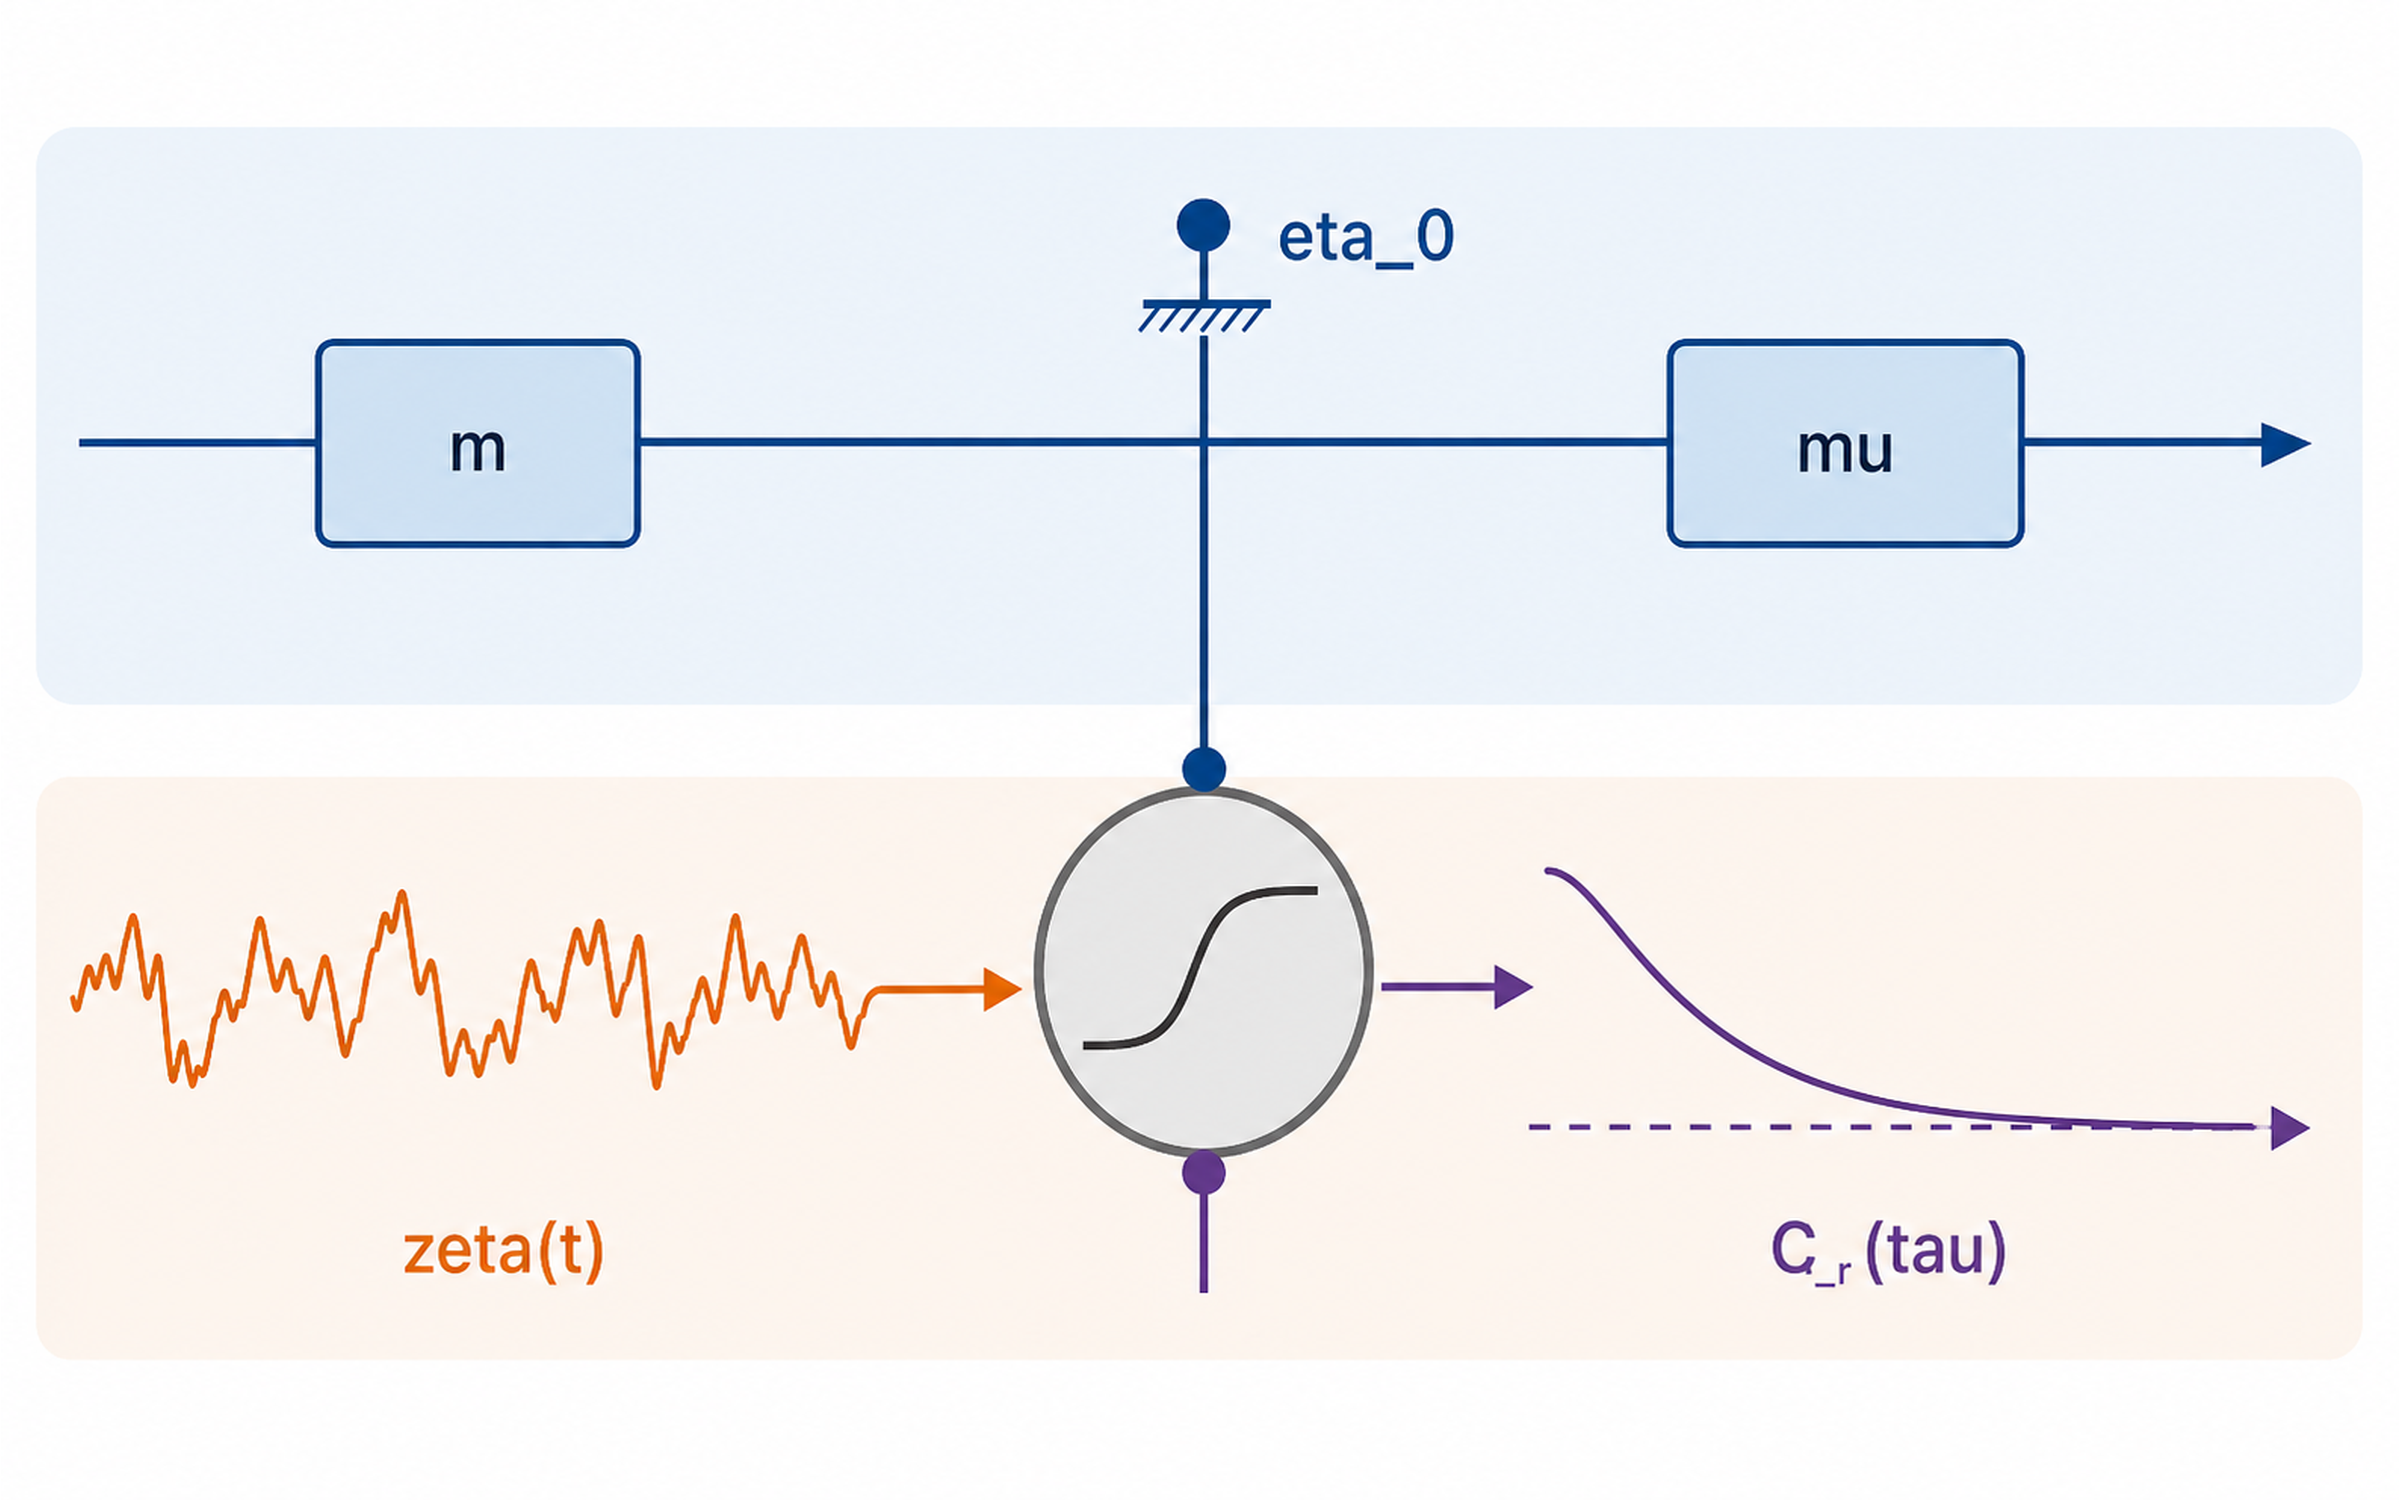
\includegraphics[width=0.88\textwidth]{figures/imagegen/ch07-static-dynamic-mean-field-split-img.png}
    \caption{Static and dynamic parts of the nonzero-mean DMFT effective process. The stationary lane contains the mean activity $m$, mean input $\mu$, and static quenched bias $\eta_0$. The connected dynamic lane contains the fluctuation process $\zeta(t)$ and its autocorrelation closure $C_r(\tau)$. Keeping these lanes separate prevents a static frozen offset from being mistaken for annealed time-dependent noise.}
    \label{fig:ch07-static-dynamic-mean-field-split}
\end{figure}

The word ``stochastic'' in this effective process is a statement about the
large-network description, not about adding external randomness to the original
deterministic rate equations. A typical unit receives many weak projections
through frozen random weights. In the \(N\to\infty\) limit, that high-dimensional
projection is summarized by a static Gaussian bias plus a Gaussian process with
the same connected autocovariance. DMFT keeps the random recurrent geometry
through the covariance closure instead of replacing it by arbitrary independent
noise.

\begin{figure}[htbp]
    \centering
    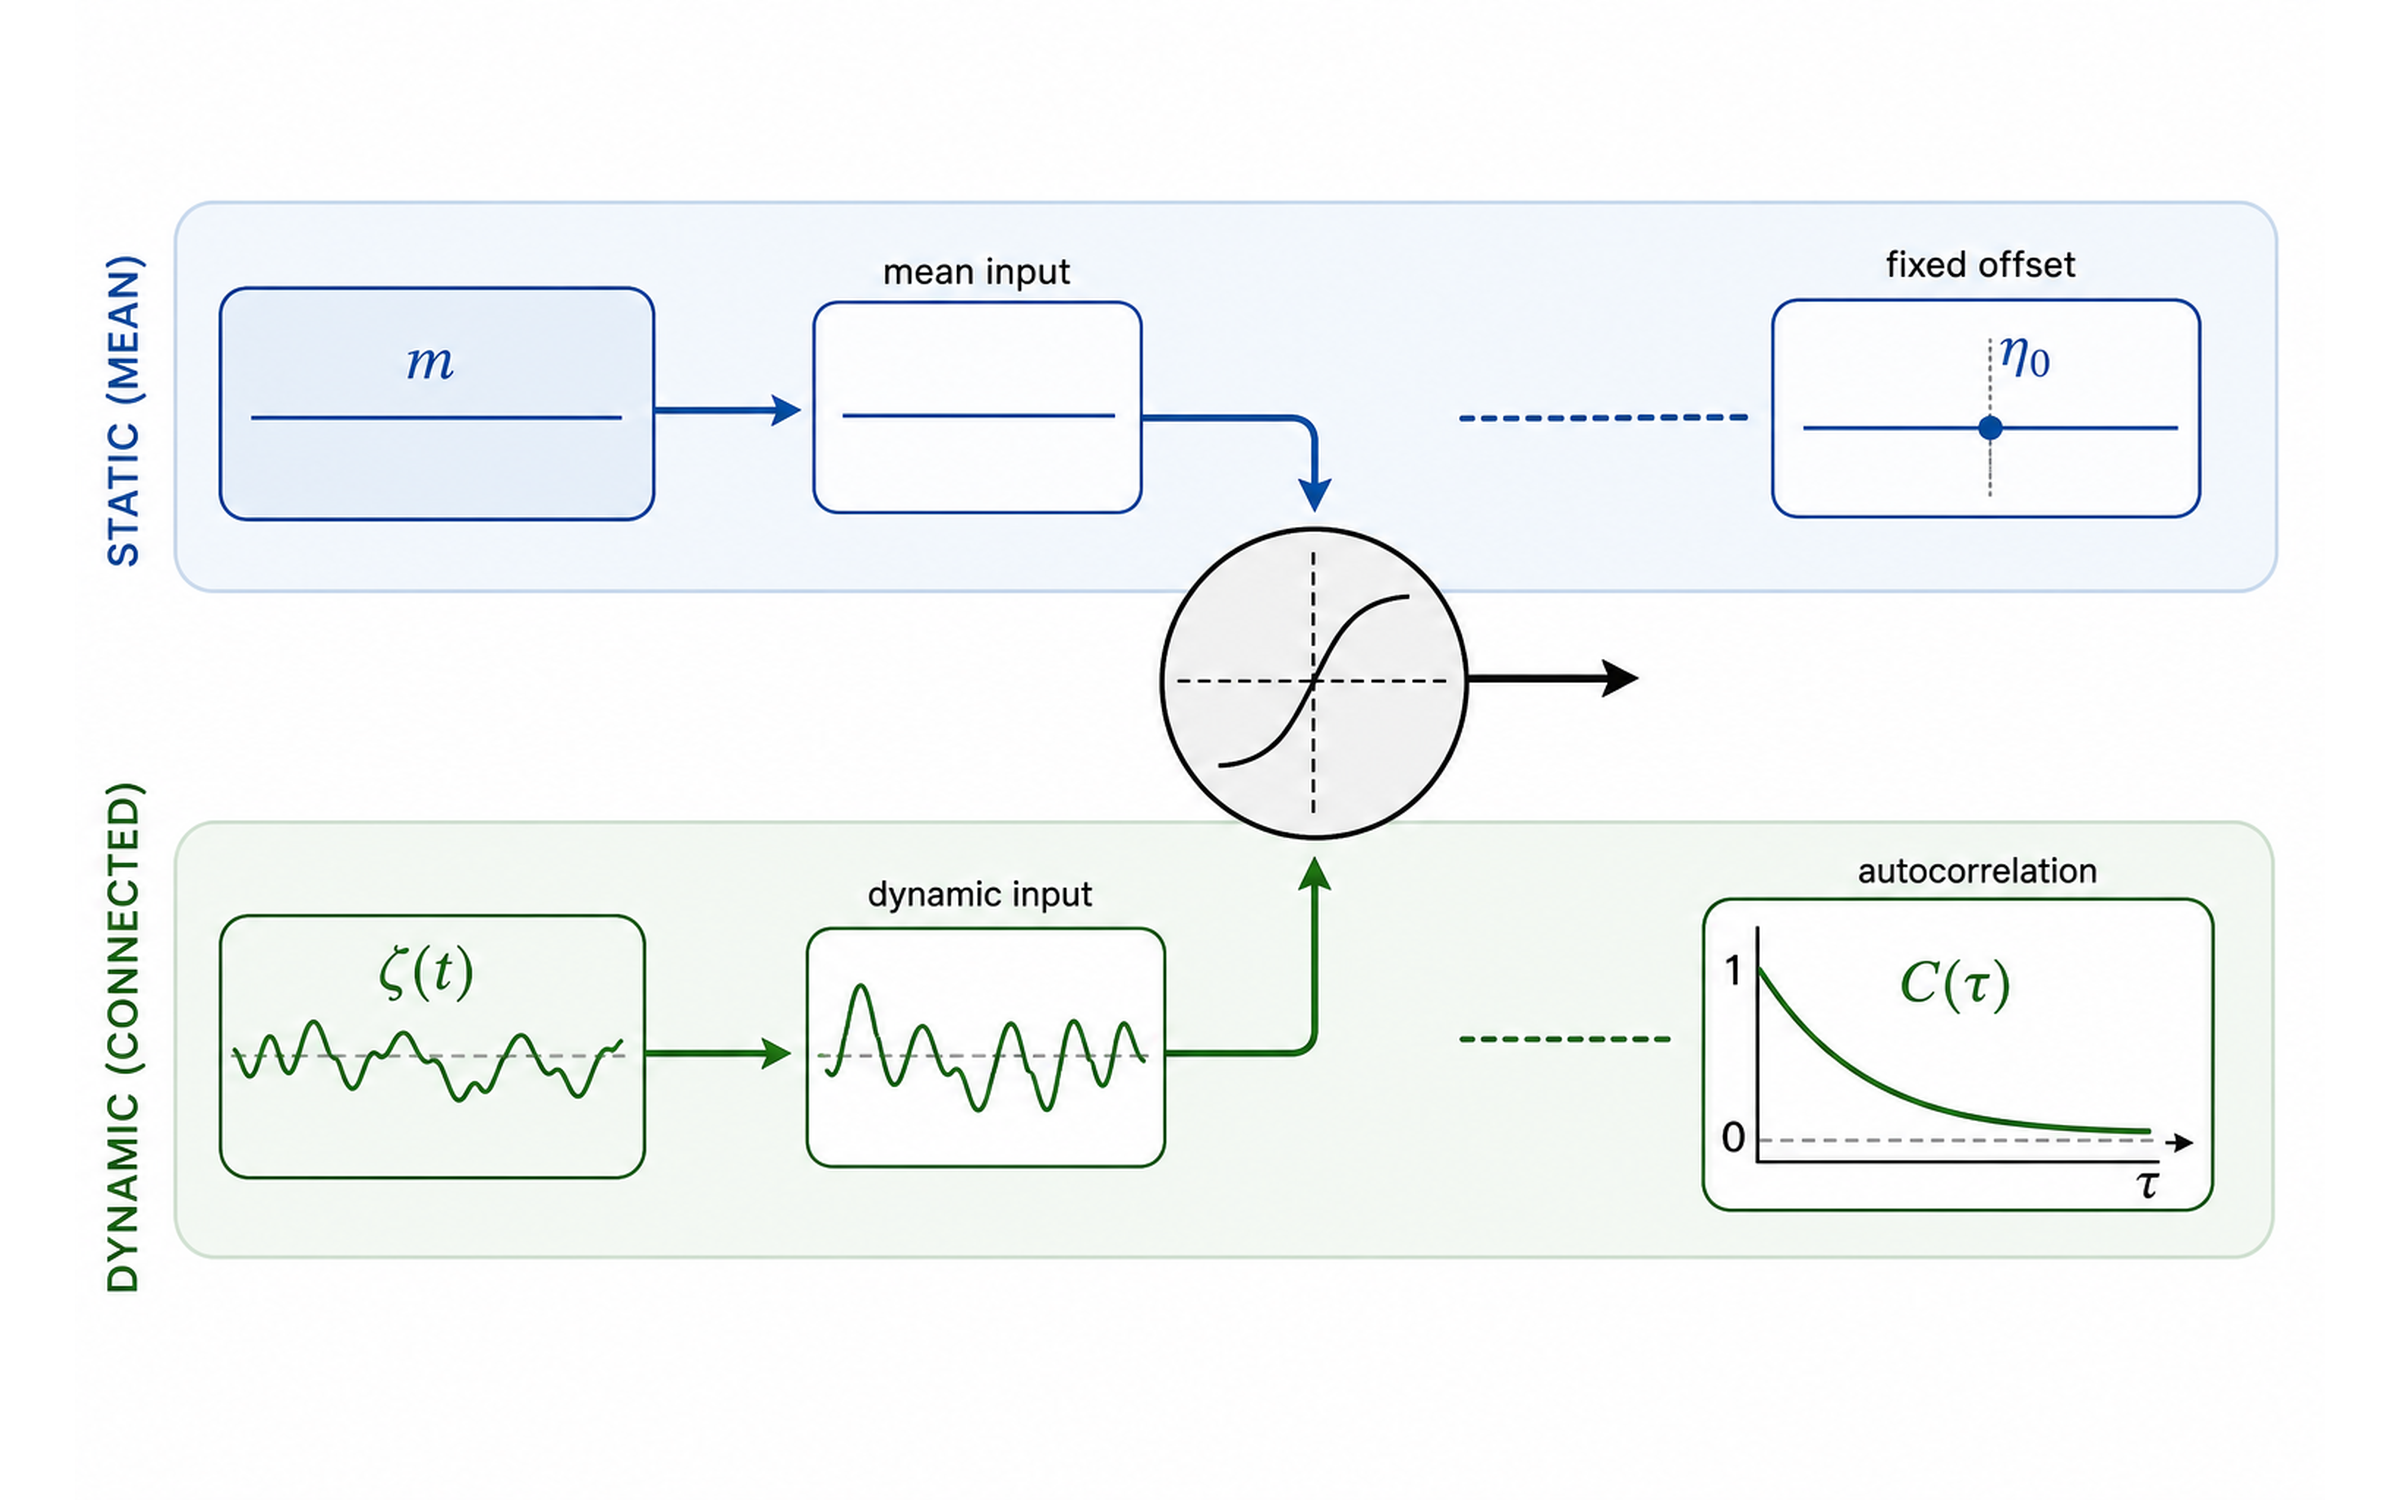
\includegraphics[width=0.88\textwidth]{figures/imagegen/ch07-dmft-self-consistency-loop-img.png}
    \caption{DMFT self-consistency loop. A high-dimensional random network is
    replaced by a representative unit driven by a mean input, a static quenched
    bias \(\eta_0\), and a connected dynamic fluctuation \(\zeta(t)\). The unit
    produces a mean rate \(m\) and connected autocorrelation \(C_r(\tau)\);
    random recurrent couplings turn these statistics into
    \(\langle\eta_0^2\rangle=g^2m^2\) and
    \(\langle\zeta(t)\zeta(t+\tau)\rangle=g^2C_r(\tau)\). The loop is closed
    only when the assumed and produced statistics agree.}
    \label{fig:ch07-dmft-self-consistency-loop}
\end{figure}

\section{Autocorrelation of Clustered Synaptic Input}
\label{sec:ch07-cluster-input-autocorrelation}

The roadmap's sparse subpopulation calculation illustrates how DMFT enters
clustered spiking networks. Let \(A_a^E(t)\) and \(A_a^I(t)\) be the
population activities in cluster \(a\). Under an infinite-cluster approximation,
different presynaptic cluster activities become asymptotically independent, so
the connected autocovariance of a sum becomes a sum of connected
autocovariances.

In the symmetric sparse setup, the connected synaptic-input autocovariance has
the form
\[
        C_y(\tau)
        =
        \left[
        \widehat J^{\,2}\left(n_E^2+g^2n_I^2\right)
        +
        \check J^{\,2}
        \left(n_E^2+\frac{g^2 f}{1-f}n_I^2\right)fK
        \right]
        C_A(\tau).
        \label{eq:ch07-roadmap-input-autocovariance}
\]
Here
\[
        C_y(\tau)
        =
        \left\langle y(t)y(t+\tau)\right\rangle-\bar{y}^{\,2},
        \qquad
        C_A(\tau)
        =
        \left\langle A(t)A(t+\tau)\right\rangle-r^2
\]
are connected autocovariances of synaptic input and population activity. Thus
the static mean contribution has already been subtracted, as in
Equation~\eqref{eq:ch07-dmft-output-covariance}; if one instead keeps raw
second moments, the static quenched term must be retained separately as in
Equation~\eqref{eq:ch07-dmft-static-quenched-bias}. The parameters \(K\),
\(f\), \(\widehat J\), and \(\check J\) have the meanings fixed above. The two
bracketed contributions have different origins. The \(\widehat J^{\,2}\) term
comes from within-cluster inputs; the \(\check J^{\,2}fK\) term comes from the
sum over connected external clusters.

For large \(K\), the external-cluster contribution dominates the
within-cluster contribution in this setup, giving the simplification
\[
        C_y(\tau)
        \approx
        \check J^{\,2}fK
        \left[
        n_E^2+\frac{g^2 f}{1-f}n_I^2
        \right]
        C_A(\tau).
        \label{eq:ch07-large-k-covariance}
\]
This equation should be read as a covariance-level analogue of balanced input.
Mean excitation and inhibition may cancel strongly, but their fluctuations and
quenched differences still shape the dynamic input statistics.

The DMFT closure is then
\[
        C_A(\tau)
        =
        \left\langle
        r(t\mid y)\,r(t+\tau\mid y)
        \right\rangle
        -
        \left\langle r(t\mid y)\right\rangle^2,
        \label{eq:ch07-spiking-dmft-closure}
\]
where \(r(t\mid y)\) is the time-dependent firing rate of a representative
neuron or population driven by the effective input process \(y(t)\). The
important point is the same as in SCS: \(C_y\) is computed from \(C_A\), and
\(C_A\) is computed from the response to \(y\).

\section{Clustered E/I Reductions}
\label{sec:ch07-ei-clustered-dmft}

For paired E/I clusters, the representative object is not a single scalar rate
but an E/I pair. Let \(A_a^\alpha(t)\) be the activity of population
\(\alpha\in\{E,I\}\) in cluster \(a\). A useful effective input decomposition is
\[
        y_a^\alpha(t)
        =
        \mu_\alpha
        +
        y_{a,\mathrm{self}}^\alpha(t)
        +
        y_{a,\mathrm{quenched}}^\alpha(t)
        +
        \xi\,y_{a,\mathrm{fs}}^\alpha(t).
        \label{eq:ch07-ei-input-decomposition}
\]
The term \(\mu_\alpha\) is the stationary balanced mean. The self term contains
potentiated within-pair couplings such as \(\widehat J^{EE}\), \(\widehat J^{EI}\),
\(\widehat J^{IE}\), and \(\widehat J^{II}\). The quenched term contains frozen
inter-cluster variability with amplitude \(\kappa\). The finite-size term has
amplitude \(\xi=1/\sqrt{n_E}\) and shrinks as cluster size grows.

A covariance-level closure must keep the E/I pair structure. Define the
connected output covariance matrix
\[
        C_{\beta\delta}(\tau)
        =
        \left\langle
        A^\beta(t)A^\delta(t+\tau)
        \right\rangle
        -
        r_\beta r_\delta,
        \qquad
        \beta,\delta\in\{E,I\}.
        \label{eq:ch07-ei-output-covariance-matrix}
\]
The diagonal entries are E and I autocovariances; the off-diagonal entries are
E/I cross-covariances. These cross-covariances matter whenever inhibitory
feedback amplifies or suppresses excitatory fluctuations, so we do not discard
them in the general closure.

As in the scalar nonzero-mean DMFT, the quenched input contains a static part
generated by the stationary rates and a dynamic connected part generated by
fluctuations around those rates. A schematic matrix closure is
\[
        \left\langle
        y_{0}^{\alpha}y_{0}^{\gamma}
        \right\rangle
        =
        \kappa^2
        \sum_{\beta,\delta\in\{E,I\}}
        M_{\alpha\gamma}^{\beta\delta}\,
        r_\beta r_\delta,
        \label{eq:ch07-ei-static-quenched-covariance}
\]
and
\[
        \left\langle
        \tilde{y}_{\mathrm{quenched}}^\alpha(t)
        \tilde{y}_{\mathrm{quenched}}^\gamma(t+\tau)
        \right\rangle
        =
        \kappa^2
        \sum_{\beta,\delta\in\{E,I\}}
        M_{\alpha\gamma}^{\beta\delta}\,
        C_{\beta\delta}(\tau).
        \label{eq:ch07-ei-quenched-covariance}
\]
Here \(y_0^\alpha\) is the static frozen bias in input channel \(\alpha\), and
\(\tilde{y}_{\mathrm{quenched}}^\alpha(t)\) is the connected dynamic
fluctuation around that bias. The coefficient tensor
\(M_{\alpha\gamma}^{\beta\delta}\) encodes the E/I architecture: connection
probabilities, signs, population sizes, and the relative strength of E and I
pathways. A diagonal approximation would set the \(\beta\ne\delta\) terms to
zero, but that approximation would erase E/I cross-covariances. In
inhibition-stabilized regimes, inhibitory pathways can strongly amplify
quenched variability because inhibitory weights are large in magnitude. This is
the mathematical reason E/I clustered networks can behave differently from
E-only clustered networks even when their mean rates look similar.

The output closure is
\[
        C_{\beta\delta}(\tau)
        =
        \left\langle
        A^\beta(t)A^\delta(t+\tau)
        \right\rangle
        -
        r_\beta r_\delta,
        \qquad
        A^\beta(t)=\Psi_\beta[y^E,y^I](t).
        \label{eq:ch07-ei-output-closure}
\]
The functional \(\Psi_\beta\) represents the population response of the
effective E/I pair to its input histories. In a rate reduction, \(\Psi_\beta\)
may be an explicit transfer function with synaptic filtering. In a spiking
DMFT, it may be defined by the stochastic LIF or GIF response to the effective
input process. Either way, the same self-consistency principle applies.

\section{Where Finite-Size Mesoscopic Theory Enters}
\label{sec:ch07-finite-size-mesoscopic-bridge}

The Schwalger-style finite-size population theory developed earlier in the
course has a different job from the SCS-style DMFT closure: it explains how a
finite population of spiking neurons becomes a noisy activity equation. In the
notation of this chapter, a schematic population activity decomposition is
\[
        A_a^\alpha(t)
        =
        \nu_a^\alpha(t)
        +
        \xi_\alpha\,\eta_{a,\xi}^\alpha(t),
        \qquad
        \xi_\alpha=\frac{1}{\sqrt{n_\alpha}},
        \label{eq:ch07-activity-finite-size-split}
\]
where \(\nu_a^\alpha(t)\) is the conditional population rate produced by the
effective input history, and \(\eta_{a,\xi}^\alpha\) is the residual finite-size
activity fluctuation. Here \(n_\alpha\) is the number of type-\(\alpha\)
neurons in the represented cluster population. The exact kernel and
colored-noise correction depend on the renewal or quasi-renewal approximation
for the LIF/GIF population, but the scaling with \(n_\alpha^{-1/2}\) is the part
needed for the present bridge.

Substituting \cref{eq:ch07-activity-finite-size-split} into the cluster input
equation separates three covariance sources:
\[
        C_y(\tau)
        =
        C_y^{\mathrm{q}}(\tau;\kappa)
        +
        \xi^2 C_y^{\mathrm{fs}}(\tau)
        +
        C_y^{\mathrm{cross}}(\tau).
        \label{eq:ch07-input-covariance-split}
\]
The deterministic or quenched term is generated by the recurrent cluster
dynamics and frozen inter-cluster structure. The finite-size term is generated
by population sampling noise and should shrink like \(1/n_E\) in covariance.
The cross term is often neglected in a first approximation, but it is a
measurable error term in simulations because finite-size fluctuations can push
the trajectory through different regions of the deterministic vector field.

This split is the bridge between the two theories. Finite-size mesoscopic
theory supplies the \(\xi\)-dependent stochastic correction to population
activity. DMFT supplies the self-consistency condition for the recurrent
deterministic and quenched input statistics. A useful reduced model must say
which part of \(C_y(\tau)\) is predicted by each mechanism.

\section{Scaling Regimes and the SCS Limit}
\label{sec:ch07-scaling-regimes-scs-limit}

The SCS analogy becomes sharp only in a many-effective-unit limit. For clustered
spiking networks, there are three distinct large-system questions:

\begin{enumerate}
    \item \emph{Fixed cluster size, many clusters.} The number of effective
    units grows, but \(\xi\) does not vanish. Irregular switching may remain
    even without deterministic mesoscopic chaos because each cluster is still a
    noisy finite population.

    \item \emph{Fixed number of clusters, large clusters.} Finite-size noise
    decreases, but there are too few effective units for a clean SCS-style
    mean-field limit. Dynamics can be strongly sample-specific because the
    frozen inter-cluster matrix has only a few rows.

    \item \emph{Many large clusters.} Both the number of effective units and
    the neurons per unit grow. This is the conceptual regime in which
    \(\xi\to0\) while the aggregate quenched inter-cluster variance remains
    order one:
    \[
        \sum_{b\ne a}
        \operatorname{Var}
        \left[
        G_{ab}\Phi(u_b)
        \right]
        =
        O(1).
        \label{eq:ch07-aggregate-quenched-variance}
    \]
    This is the closest analogue of the SCS thermodynamic limit and the most
    direct route to deterministic mesoscopic chaos.
\end{enumerate}

These regimes should not be collapsed into a single phrase such as large
network. The first preserves finite-size fluctuations, the second removes
them but lacks a population of effective units, and the third is the intended
DMFT bridge between random rate chaos and paired E/I clusters.

\section[The xi-kappa Interpretation]{The \(\xi\)-\(\kappa\) Interpretation}
\label{sec:ch07-xi-kappa}

The two-parameter view \((\xi,\kappa)\) organizes the central distinction in the
roadmap. The finite-size coordinate
\[
        \xi = \frac{1}{\sqrt{n_E}}
\]
measures sampling noise in cluster activity. The quenched coordinate
\(\kappa\) measures frozen inter-cluster variability. The two limits answer
different questions.

If \(\kappa\) is small and switching disappears as \(\xi\to 0\), the switching
was driven by finite cluster size. This is the multistable-attractor picture:
large clusters reveal stable attractors because the noise that kicked the system
between basins has vanished.

If switching persists as \(\xi\to 0\) at nonzero \(\kappa\), then finite-size
noise is not the source of the switching. The remaining candidate is
deterministic mesoscopic chaos generated by the frozen inter-cluster structure.
In that regime, switch times should plateau as \(n_E\) grows, and the
autocorrelation should have the smooth zero-lag shape expected of deterministic
chaotic rate dynamics rather than a finite-size kink.

\section{Reading Map for the Course Ladder}
\label{sec:ch07-reading-map}

The literature is most useful when each paper family is attached to a modeling
operation in the course rather than treated as a separate reading list.

\begin{center}
\renewcommand{\arraystretch}{1.35}
\begin{tabularx}{\textwidth}{@{}p{0.22\textwidth}p{0.21\textwidth}X@{}}
  \toprule
  \textbf{Source family} & \textbf{Course anchor} & \textbf{What to extract for rotation work} \\
  \midrule
  Brunel balanced networks & Ch04, Ch08 & How sparse E/I recurrence, fixed in-degree choices, and external drive create an asynchronous irregular baseline before clustering is added. \\
  van Vreeswijk--Sompolinsky balance & Ch04, Ch07 & Why excitation and inhibition can be individually large while their mean cancels, and why fluctuations remain dynamically important. \\
  Litwin-Kumar--Doiron clustered balance & Ch05, Ch09 & How clustered excitation creates slow active-set switching that is naturally tested by finite-size scaling. \\
  Mazzucato-style metastability & Ch05, Ch09, Ch10 & How to measure active clusters, lifetimes, Fano factors, and low-dimensional state structure without immediately calling the result chaos. \\
  Schwalger finite-size population theory & Ch03, Ch07 & How LIF/GIF spike trains become noisy mesoscopic activity equations with explicit \(1/\sqrt{N}\) population fluctuations. \\
  SCS and dynamic mean-field theory & Ch06, Ch07, Ch09 & How random recurrent gain creates deterministic rate chaos, and why autocorrelation self-consistency and Lyapunov tests are the core diagnostics. \\
  Stern--Sompolinsky--Abbott self-coupled units & Ch06, Ch08 & How local self-coupling or bistability inside each unit changes the route from random recurrence to switching or chaos. \\
  Rostami/Tilo paired E/I clusters & Ch08, Ch09, Ch10 & How paired excitatory and inhibitory clusters turn the abstract SCS/DMFT mechanism into an implementable spiking-network research program. \\
  \bottomrule
\end{tabularx}
\end{center}

Read in that order, the papers form a ladder: balance gives the operating
point, clustering gives metastable units, finite-size theory explains noisy
population activity, SCS/DMFT explains deterministic recurrent chaos, and the
paired E/I model asks which mechanism survives the \((\xi,\kappa)\) tests.

\section{What Carries Forward}
\label{sec:ch07-carries-forward}

The chapters that follow use the DMFT language developed here to interpret
paired E/I clusters, scaling tests, perturbation tests, and phase diagrams. The
main points are:

\begin{enumerate}
    \item Static mean field matches stationary rates and stationary balanced
    input.
    \item DMFT matches autocorrelations and effective stochastic input
    processes.
    \item Quenched disorder is frozen recurrent structure, not merely added
    noise.
    \item The \((\xi,\kappa)\) plane separates finite-size switching from
    quenched-disorder-driven mesoscopic chaos.
    \item Cluster activities can be effective rate units while still retaining
    spiking information through transfer functions, finite-size noise, synaptic
    filtering, and E/I covariance structure.
\end{enumerate}

\begin{chaptersummary}
\begin{center}
\renewcommand{\arraystretch}{1.35}
\begin{tabularx}{\textwidth}{@{}l X X@{}}
  \toprule
  \textbf{Layer} & \textbf{Closure} & \textbf{Diagnostic consequence} \\
  \midrule
  Static mean field &
  \(r_\alpha=\Phi_\alpha(\mu_\alpha)\) &
  Checks stationary balance and baseline rates \\
  SCS DMFT &
  \(\langle\zeta(t)\zeta(t+\tau)\rangle=g^2C_r(\tau)\) &
  Predicts autocorrelation in a random rate network \\
  Nonzero-mean DMFT &
  Static bias \(g^2m^2\) plus connected covariance \(g^2C_r(\tau)\) &
  Prevents frozen offsets from being mistaken for time-dependent noise \\
  E/I cluster DMFT &
  \(C_y^{\alpha\gamma}(\tau)=
  \sum_{\beta\delta}M_{\alpha\gamma}^{\beta\delta}
  C_{\beta\delta}(\tau)\) &
  Keeps E/I cross-covariances and inhibitory amplification visible \\
  Finite-size bridge &
  \(A_a^\alpha=\nu_a^\alpha+\xi_\alpha\eta_{a,\xi}^\alpha\) &
  Predicts which covariance components should shrink with cluster size \\
  \bottomrule
\end{tabularx}
\end{center}
\end{chaptersummary}

\section{Contribution-Level Checkpoints}
\label{sec:ch07-contribution-checkpoints}

\begin{enumerate}
    \item Starting from \cref{eq:ch08-population-drive}, derive a two-type
    version of \cref{eq:ch07-ei-quenched-covariance} for a simplified model
    with independent inter-cluster weight perturbations. Identify which terms
    are lost if \(C_{EI}(\tau)\) and \(C_{IE}(\tau)\) are set to zero.

    \item Simulate the effective process
    \cref{eq:ch07-dmft-effective-rate} with a guessed covariance, estimate the
    output \(m\) and \(C_r(\tau)\), and iterate the covariance update. Compare
    the converged autocorrelation with a direct finite-\(N\) SCS simulation.

    \item For one clustered spiking simulation, estimate the decomposition in
    \cref{eq:ch07-input-covariance-split} across at least two cluster sizes.
    Report which component scales like \(1/n_E\), which component remains
    fixed by the quenched realization, and whether cross terms are negligible.

    \item Run paired perturbation tests under three conditions: same quenched
    matrix and common finite-size noise, same quenched matrix and independent
    finite-size noise, and redrawn quenched matrix. Explain which condition is
    relevant for a Lyapunov claim and which conditions answer different
    stochastic robustness questions.

    \item Write a one-page model-comparison memo using the reading map:
    specify which equations come from balance, which from finite-size
    population theory, which from SCS/DMFT, and which remain implementation
    choices in the paired E/I clustered network.
\end{enumerate}
